\section{Vision Transformer基本原理}
\subsection{经典Transformer}
Transformer 模型最初由 Google Brain 团队提出，其核心创新在于引入自注意力机制（Self-Attention Mechanism），有效建模序列中各位置之间的长距离依赖关系。相较于传统循环神经网络（RNN），该机制不仅提高了特征提取能力，还显著增强了模型的并行计算能力，从而提升了训练效率与表现效果。

Transformer 最初被广泛应用于自然语言处理领域，尤其在机器翻译任务中取得了突破性成果。然而，得益于其强大的表示能力与高度的架构灵活性，Transformer 很快被扩展至计算机视觉等多个领域。本文将首先简要回顾经典的 Transformer 模型架构及其原理\supercite{vaswaniAttentionAllYou2017}。
\subsubsection{注意力机制}
在注意力机制的背景下，自主性提示被称为查询($\boldsymbol{q} \in \mathbb{R}^{q}$)，非自主性提示被称为键($\boldsymbol{k}\in \mathbb{R}^{k}$)。
注意力汇聚将给定的查询与键进行匹配，最终根据所得的注意力权重得出最匹配的值。
\begin{figure}[H]
  \centering
  \begin{subfigure}[b]{0.48\textwidth}
    \centering
    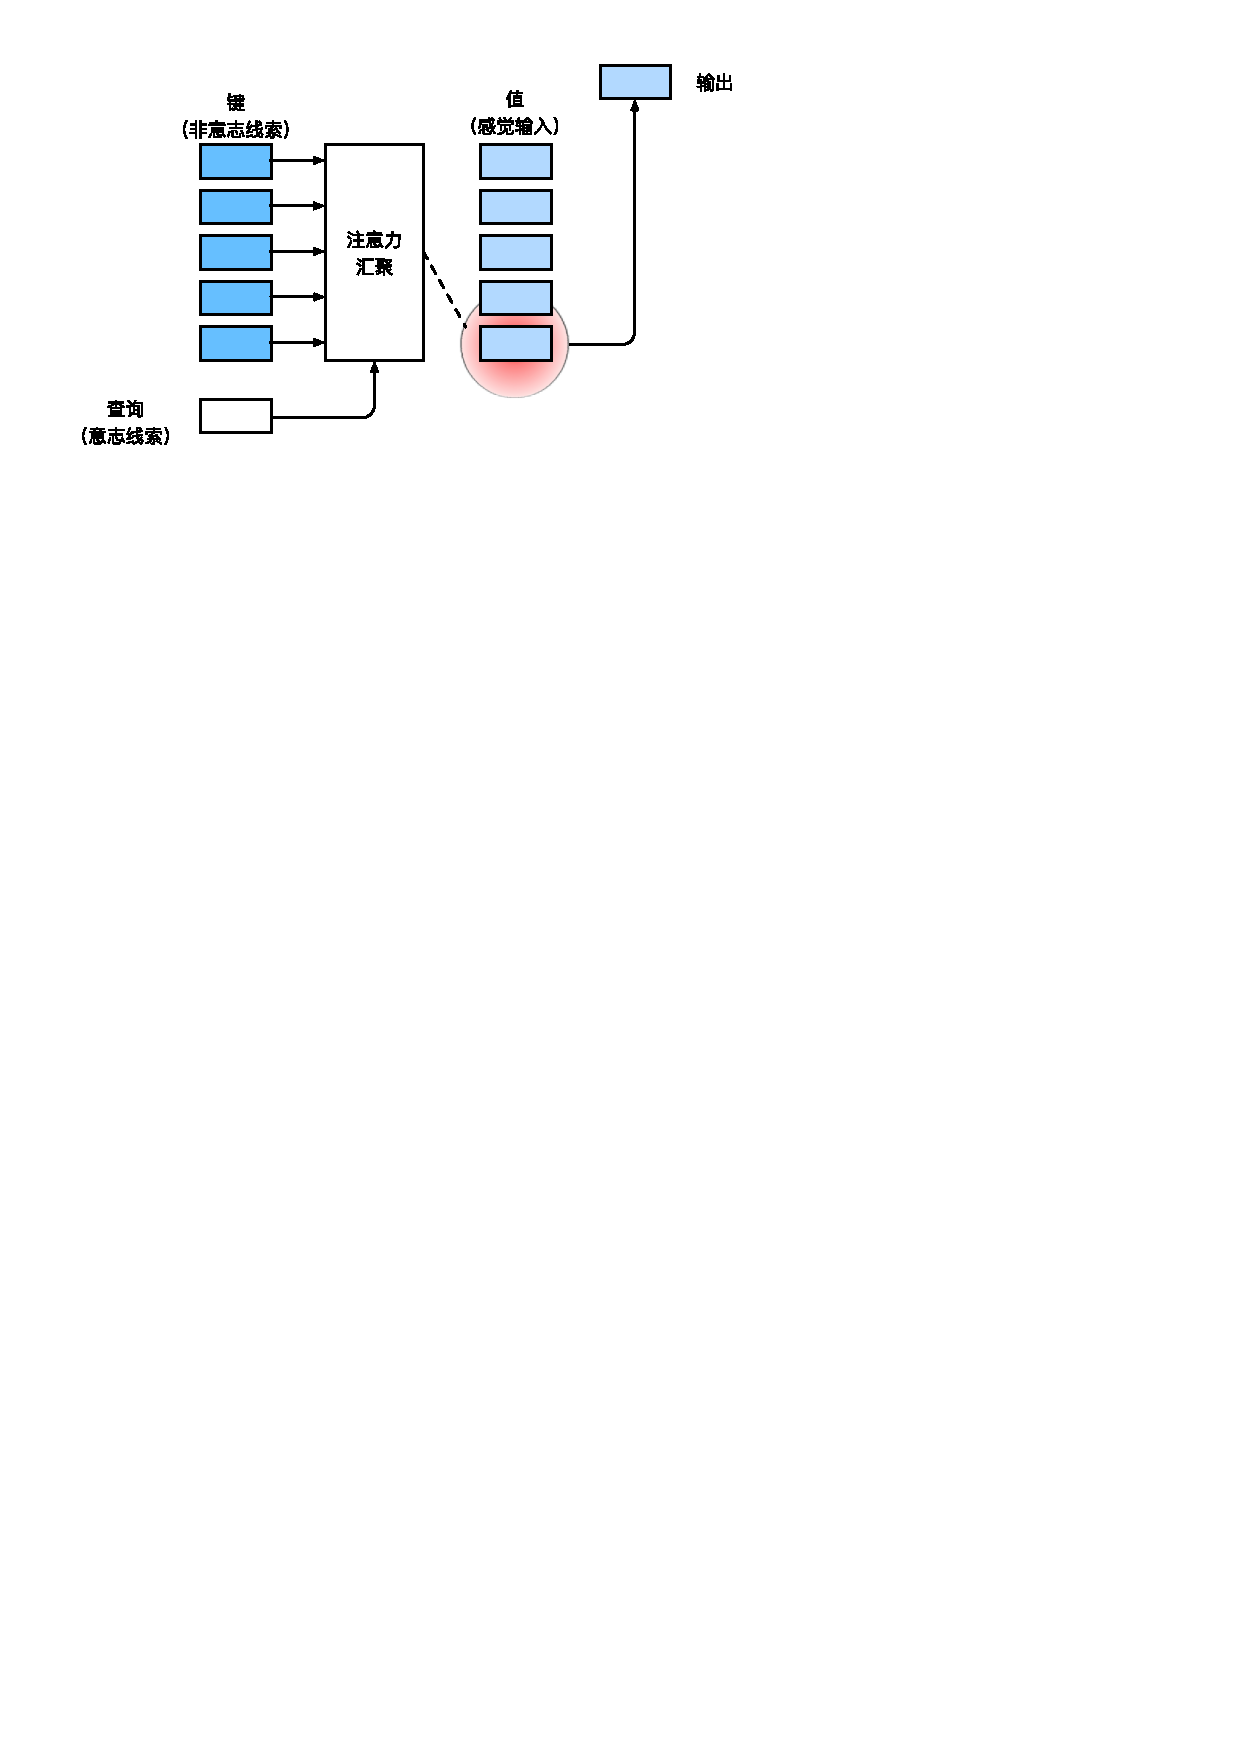
\includegraphics[width=\linewidth, height=0.2\textheight, keepaspectratio]{pic/qkv}
    \caption{注意力机制图示}
    \label{fig:qkv}
  \end{subfigure}
  \hfill
  \begin{subfigure}[b]{0.48\textwidth}
    \centering
    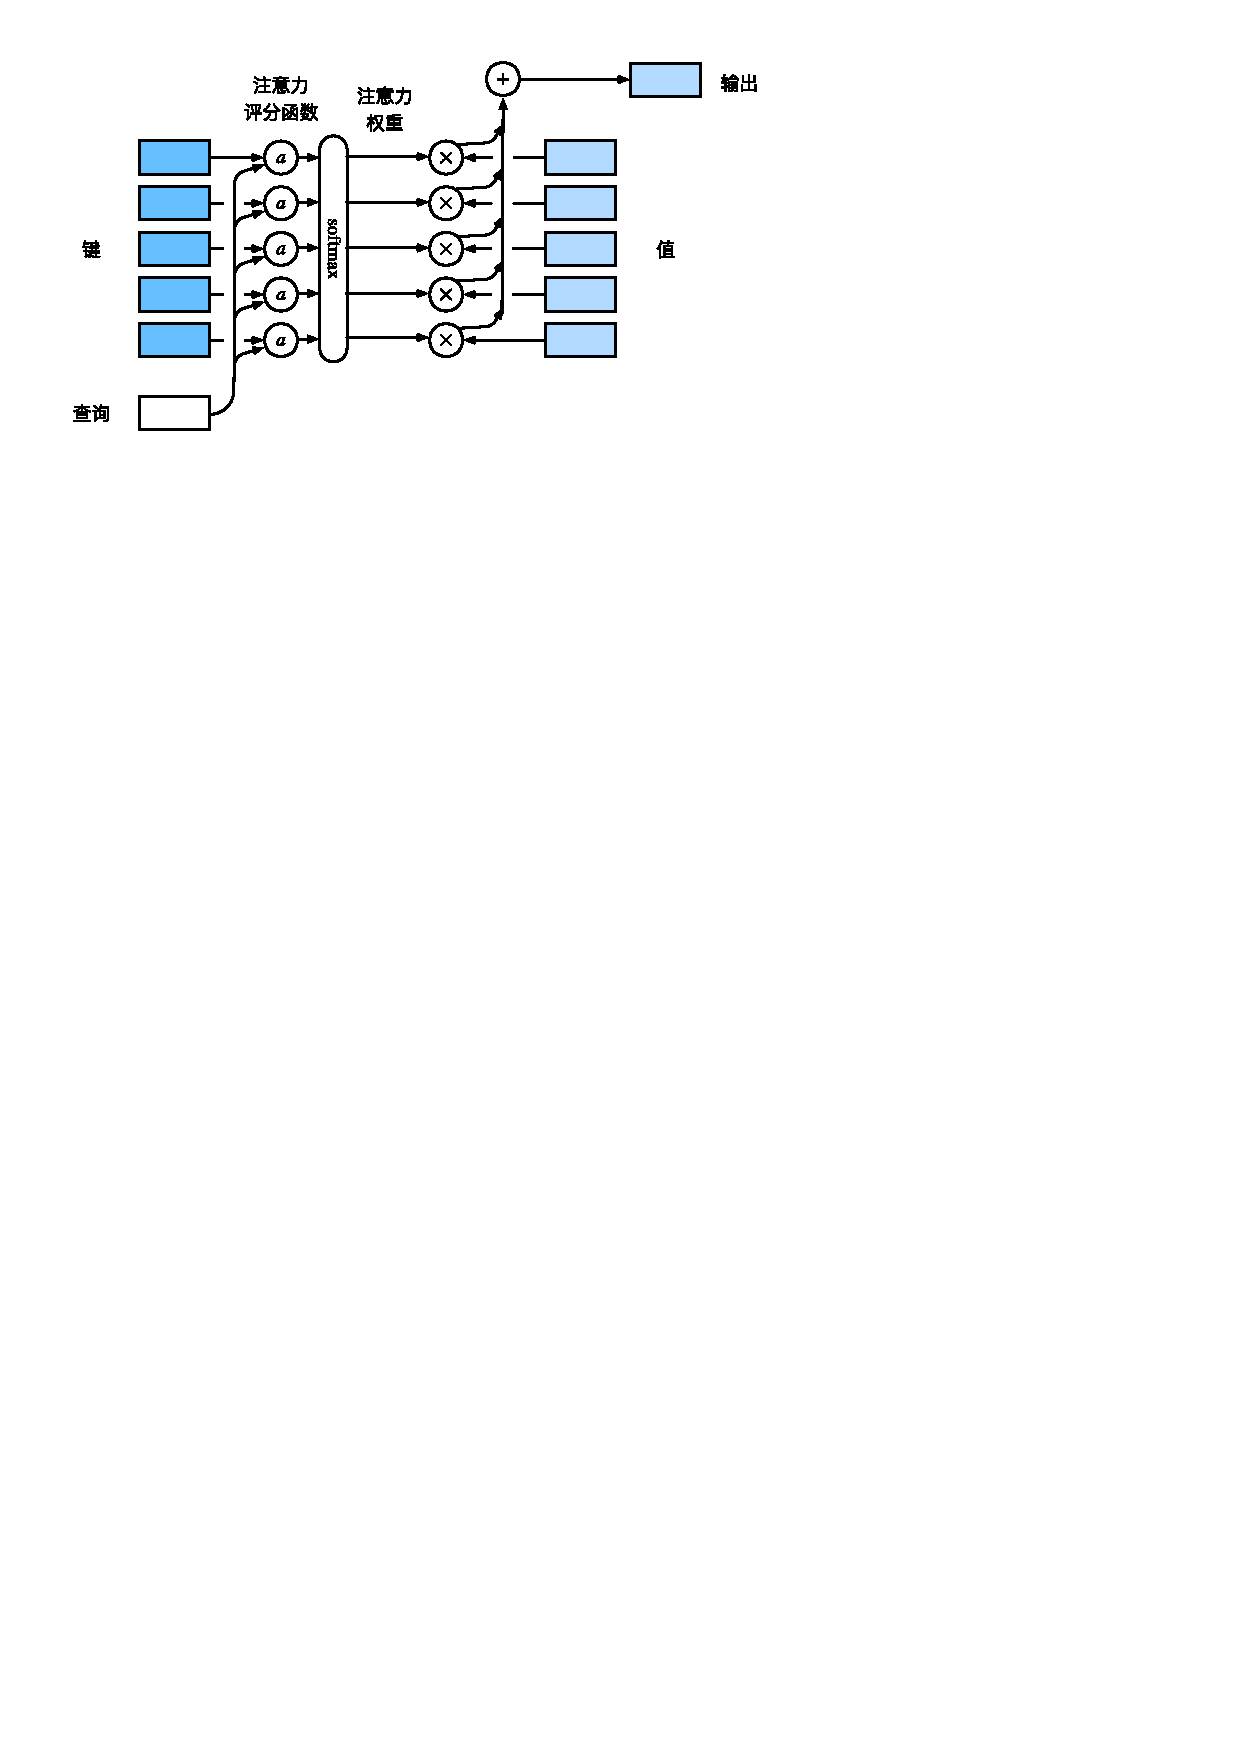
\includegraphics[width=\linewidth, height=0.2\textheight, keepaspectratio]{pic/attention-output}
    \caption{注意力汇聚的输出为值的加权和}
    \label{fig:attention}
  \end{subfigure}
  \caption{注意力机制示意}
  \label{fig:qkv_attention}
\end{figure}
通常用$f\left(\boldsymbol{q}, \boldsymbol{k}, \boldsymbol{v}\right) \in \mathbb{R}$
、$a\left(\boldsymbol{q}, {k}_{i}\right) \in \mathbb{R}$
和$\alpha\left(\boldsymbol{q}, {k}_{i}\right) \in \mathbb{R}$
分别表示注意力汇聚、注意力评分函数和注意力权重，则注意力汇聚函数$f$可表示为值的加权和：
            \begin{equation}
                f\left(\boldsymbol{q}, \boldsymbol{k}, \boldsymbol{v}\right)
                = \sum_{i=1}^{n} \alpha\left(\boldsymbol{q}, {k}_{i}\right) {v}_{i}
                = \sum_{i=1}^{n} \operatorname{softmax}\left(a(\boldsymbol{q}, {k}_{i})\right) {v}_{i}\label{eq:attention-aggregation}
            \end{equation}
\begin{enumerate}[label={（\arabic*）}, leftmargin=2em, labelsep=0.5em, itemsep=0pt]
    \item 当查询和键的长度不同时（不妨设$\boldsymbol{q} \in \mathbb{R}^{q}$、$\boldsymbol{k} \in \mathbb{R}^{k}$），可以使用加性注意力作为评分函数：
    \begin{equation}
a(\boldsymbol{q}, \boldsymbol{k})=\boldsymbol{w}_v^{\top} \tanh \left(\boldsymbol{W}_q \boldsymbol{q}+\boldsymbol{W}_k \boldsymbol{k}\right) \in \mathbb{R}\label{eq:additive-attention}
    \end{equation}
    其中$\boldsymbol{W}_q \in \mathbb{R}^{m \times q}$、$\boldsymbol{W}_k \in \mathbb{R}^{m \times k}$ 和 $\boldsymbol{w}_v \in \mathbb{R}^{m}$ 可学习。
    加性注意力将查询与键分别线性投影后相加，再输入一个仅含单个隐藏层（隐藏单元数为 $m$）且禁用偏置项的感知机；此处 $m$ 为该隐藏层维度，与后文多头注意力中的头数 $h$ 含义不同。
    \item 在点积操作中，设查询和键的维度均为 $d$（在多头注意力中即每个头的键维度 $d_{\text{model}}/h$），且其各分量相互独立、均值为 $0$、方差为 $1$，则两向量点积的均值为 $0$、方差为 $d$。可以通过除以 $\sqrt{d}$ 缩放点积结果，以避免梯度消失或爆炸问题：
        \begin{align}
            &a(\boldsymbol{q}, \boldsymbol{k})=\frac{\boldsymbol{q}^{\top} \boldsymbol{k}}{\sqrt{d}} \in \mathbb{R}
            \Rightarrow
            \operatorname{Attention}(\boldsymbol{Q}, \boldsymbol{K}, \boldsymbol{V})
            = \operatorname{softmax}\left(\frac{\boldsymbol{Q}\boldsymbol{K}^{\top}}{\sqrt{d}}\right) \boldsymbol{V}.
        \end{align}
    \item 掩蔽 softmax 通过将被掩蔽的位置替换为一个极大的负数，从而在 softmax 后将相应的权重压缩为接近 0。这一机制能够有效屏蔽不相关位置，仅关注输入序列中指定范围内的重要信息。
    \begin{figure}[H]
        \centering
        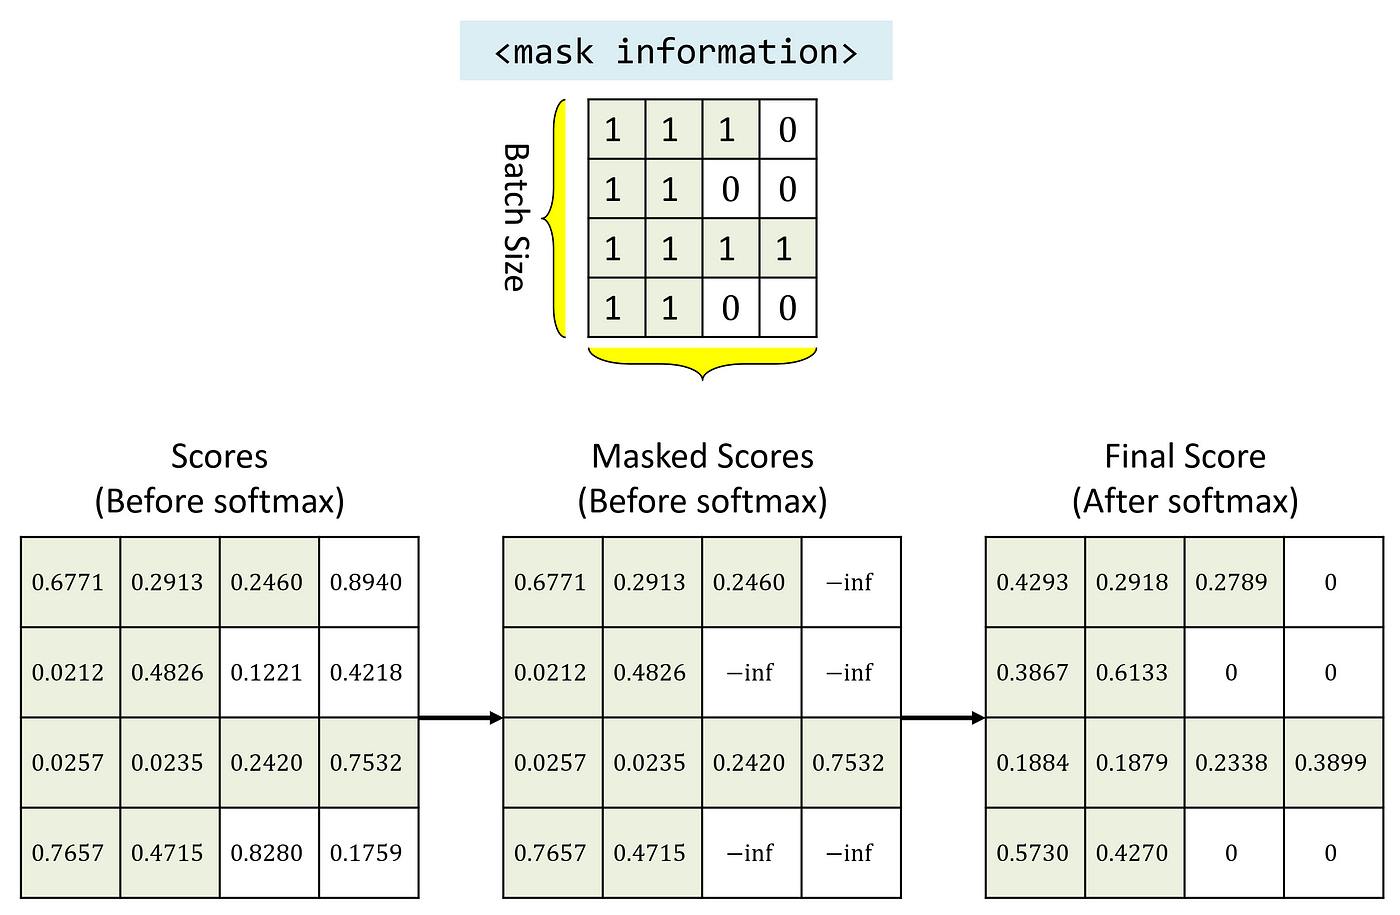
\includegraphics[width=0.6\textwidth, height=0.15\textheight, keepaspectratio]{pic/masked-softmax}
        \caption{掩蔽 softmax，其中任何超出有效长度的位置都被掩蔽并置为 0}
        \label{fig:figure2}
    \end{figure}
    常见的掩码类型包括：
\begin{enumerate}[label={（\alph*）}, leftmargin=2em, labelsep=0.5em, itemsep=0pt]
\item 填充掩码（Padding Mask）：为对齐不同长度的序列，通常在较短序列的末尾添加填充符（padding token）。填充掩码用于在注意力计算中屏蔽这些位置，避免模型关注无效信息。
\item 序列掩码（Sequence Mask）：用于根据任务需求屏蔽输入序列中的特定位置，防止模型处理无效或不相关的信息。例如，在双向模型中，可通过掩码忽略特定上下文，从而更灵活地控制信息流动。
\item 前瞻掩码（Look-ahead Mask）：又称因果掩码（Causal Mask），用于自回归模型中，屏蔽当前位置之后的信息，确保模型仅利用当前位置及之前的输入进行预测，防止未来信息泄漏。
\end{enumerate}
    \item 多头注意力机制通过多个注意力头的并行计算，使模型能够在不同的表示子空间中学习序列中各位置之间的关联，从而在相同注意力结构下捕捉多种范围的依赖关系，提升特征表示的丰富性与建模能力，其结构与计算方式如图~\ref{fig:figure3} 所示。其中第 $i$ 个头通过可学习的投影矩阵 $\boldsymbol{W}_i^{(Q)},\boldsymbol{W}_i^{(K)},\boldsymbol{W}_i^{(V)}$ 将查询、键、值映射到各自的子空间后再计算注意力，各头输出沿特征维度拼接后，由输出投影矩阵 $\boldsymbol{W}^{(O)}$ 融合为最终表示。
    \begin{figure}[H]
      \centering
      \begin{minipage}[c]{0.2\textwidth}
        \centering
        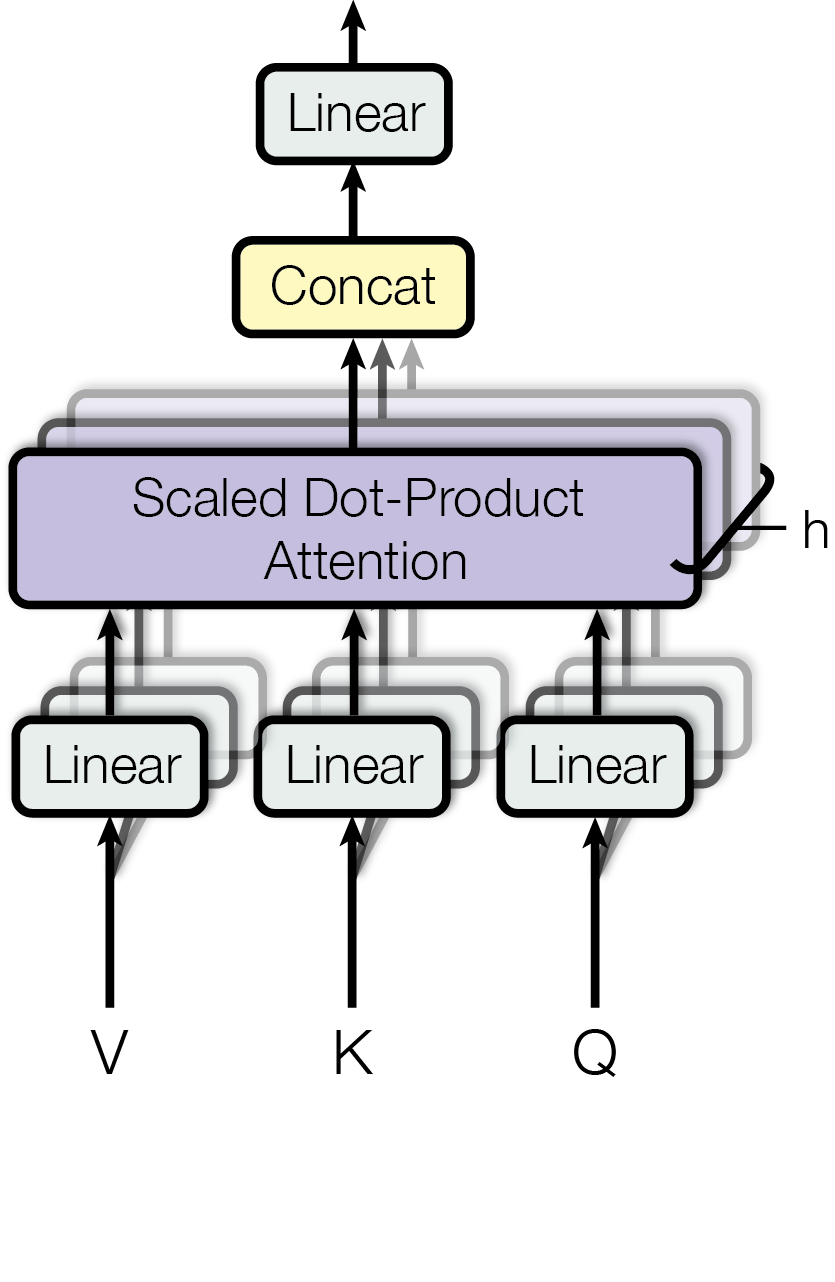
\includegraphics[width=\textwidth, keepaspectratio]{pic/ModalNet-20}
      \end{minipage}%
      \hfill
      \begin{minipage}[c]{0.8\textwidth}
        \begin{align}
          &\text{MultiHead}(\boldsymbol{Q}, \boldsymbol{K}, \boldsymbol{V}) = \text{Concat}(\boldsymbol{h}_1, \dots, \boldsymbol{h}_h)\,\boldsymbol{W}^{(O)}, \\
          &\boldsymbol{h}_{i} = \text{Attention}\left(\boldsymbol{Q}\boldsymbol{W}_{i}^{(Q)}, \boldsymbol{K}\boldsymbol{W}_{i}^{(K)}, \boldsymbol{V}\boldsymbol{W}_{i}^{(V)}\right) \\
          &\text{Attention}(\boldsymbol{Q}, \boldsymbol{K}, \boldsymbol{V}) = \text{softmax}\left(\frac{\boldsymbol{Q} \boldsymbol{K}^{\top}}{\sqrt{d}}\right) \boldsymbol{V}
        \end{align}
      \end{minipage}
      \caption{多头缩放点积注意力}
      \label{fig:figure3}
    \end{figure}
    \item 若查询、键和值均由同一组输入经各自的线性投影得到，则该注意力称为自注意力。记输入序列为 $\boldsymbol{X}$，即取 $\boldsymbol{Q}=\boldsymbol{X}\boldsymbol{W}^{(Q)}$、$\boldsymbol{K}=\boldsymbol{X}\boldsymbol{W}^{(K)}$、$\boldsymbol{V}=\boldsymbol{X}\boldsymbol{W}^{(V)}$；若略去投影、直接以 $\boldsymbol{X}$ 充当查询、键、值，则可简化表示为：
    \begin{equation}
        \text{Attention}\left(\boldsymbol{X}, \boldsymbol{X}, \boldsymbol{X}\right) =\text{softmax}\left(\frac{\boldsymbol{X} \boldsymbol{X}^{\top}}{\sqrt{d}}\right) \boldsymbol{X}
    \end{equation}
    \item 为了使模型能够利用序列的顺序，可通过在输入嵌入中添加位置编码来引入绝对或相对的位置信息。
    位置编码可以通过学习得到，也可以直接固定得到。
    以正余弦位置编码这一固定位置编码方式为例，假设$\boldsymbol{X} \in \mathbb{R}^{n \times d}$表示一个序列中$n$个位置（如$n$个词元）的$d$维嵌入表示，则位置编码使用相同形状的位置嵌入矩阵$\boldsymbol{P} \in \mathbb{R}^{n \times d}$，输出
    $\boldsymbol{X}+ \boldsymbol{P}$，其中：
    \begin{align}
    PE_{pos,2i}&=\sin\left( pos/10000^{2i/d}\right), \quad PE_{pos,2i+1}&=\cos\left( pos/10000^{2i/d}\right)
    \end{align}
\end{enumerate}

\subsubsection{经典Transformer架构}
Transformer 模型由多个编码器（Encoder）和解码器（Decoder）模块交替堆叠而成，其中编码器负责对输入序列进行建模，提取全局特征；解码器则在此基础上生成目标输出序列。
\begin{figure}[H]
    \centering
    \begin{subfigure}[b]{0.5\textwidth}
        \centering
        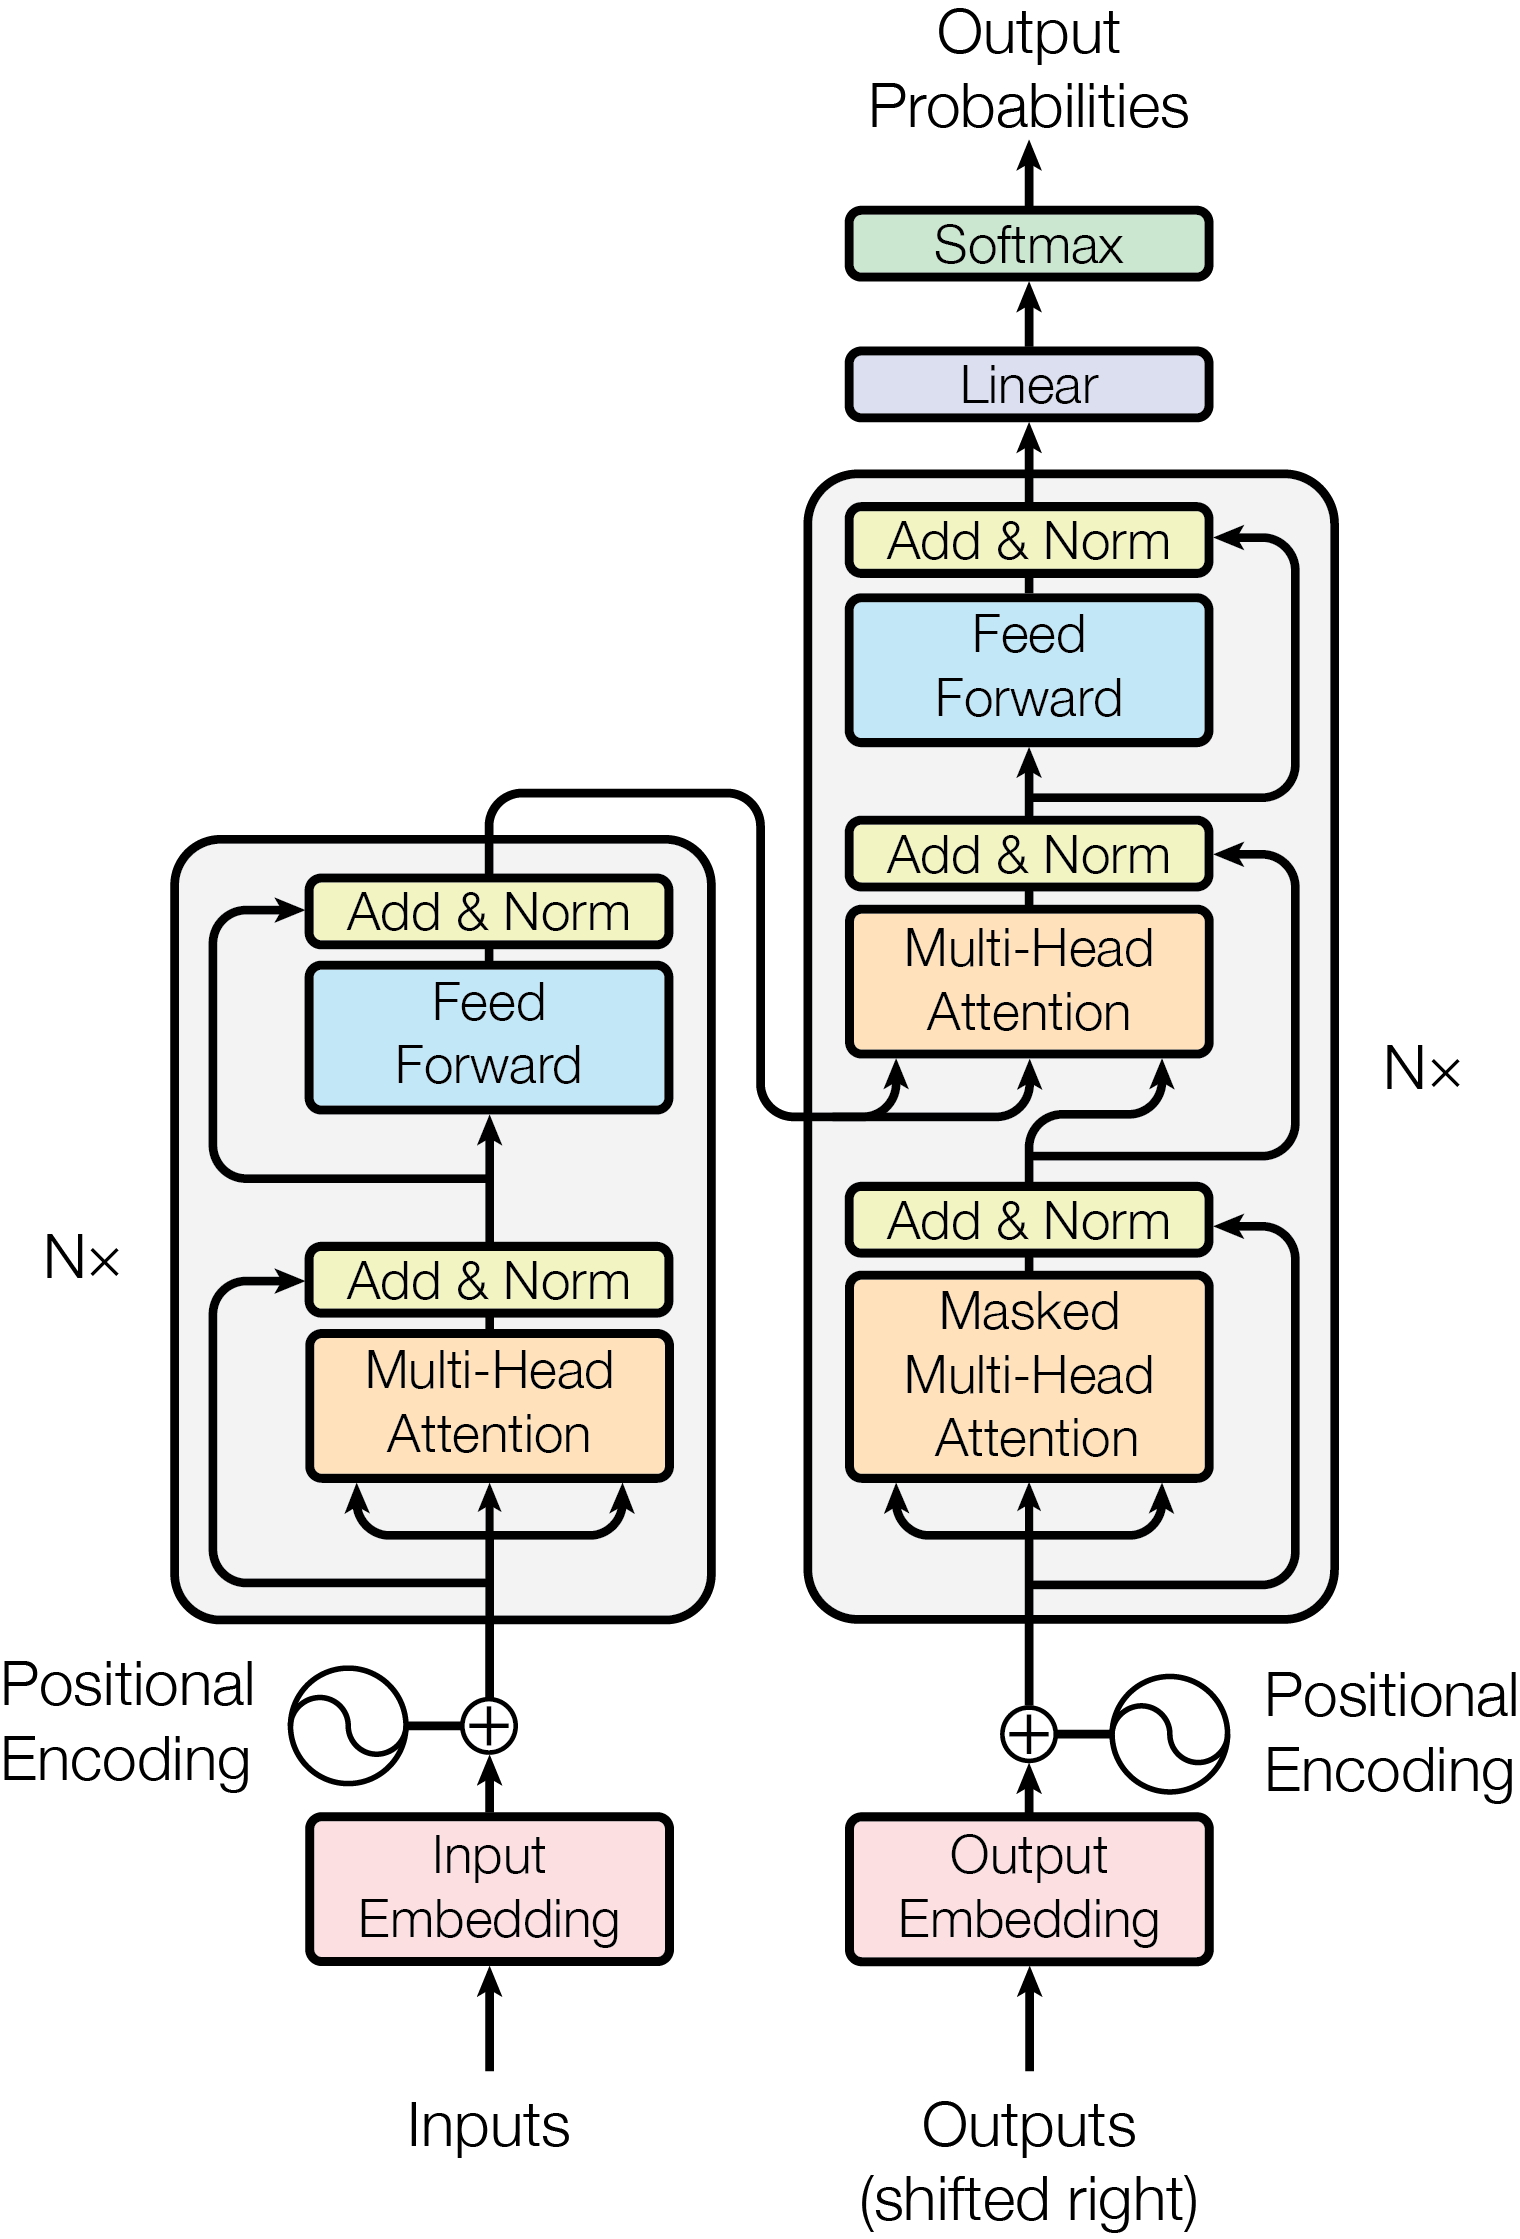
\includegraphics[width=\linewidth, height=0.3\textheight, keepaspectratio]{pic/ModalNet-21}
        \caption{Transformer 整体架构}
        \label{fig:transformer-arch}
    \end{subfigure}
    \hfill
    \begin{subfigure}[b]{0.48\textwidth}
        \centering
        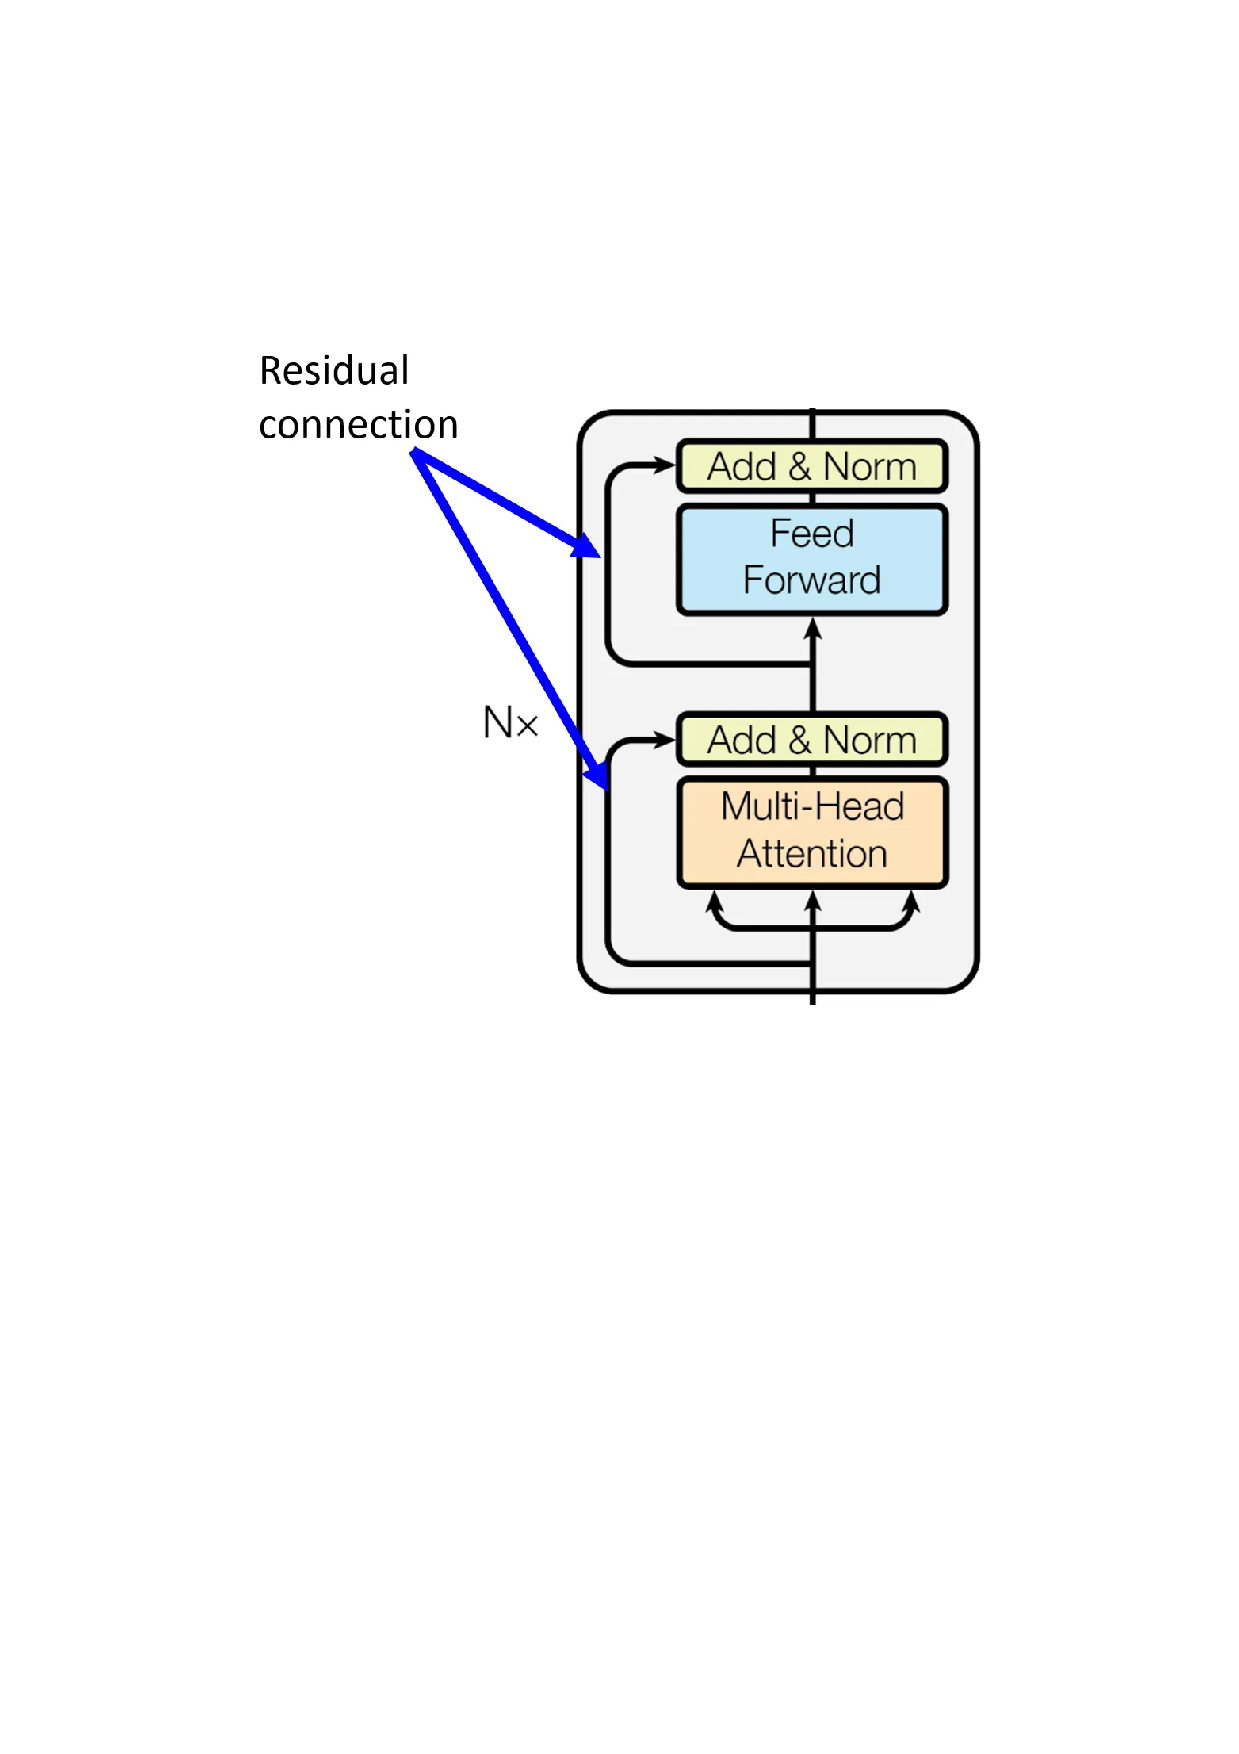
\includegraphics[width=\linewidth, height=0.3\textheight, keepaspectratio]{pic/residual_connection}
        \caption{残差连接}
        \label{fig:residual}
    \end{subfigure}
    \caption{Transformer 架构与残差连接}
    \label{fig:transformer}
\end{figure}
编码器的每一层主要由两部分构成：多头自注意力（Multi-head Self-Attention）机制和基于位置的前馈神经网络（Position-wise Feed-Forward Network）。

解码器则在保留上述结构的基础上，额外引入编码器-解码器注意力（Encoder-Decoder Attention）机制，以实现对编码器输出的动态关注，从而更有效地建模输入与输出之间的对齐关系。

对于Transformer模型中涉及的多种注意力，其查询（Query）、键（Key）和值（Value）的来源分别如表\ref{tab:attn-structure-simple}所示：
\begin{table}[H]
    \centering
    \caption{Transformer 中各注意力模块的输入结构}
    \begin{tabular}{ccc}
        \toprule
        \textbf{模块} & \textbf{注意力类型} & \textbf{Query / Key / Value 的来源} \\
        \midrule
        编码器 & 多头自注意力 & 编码器前一层的输出 / 同 / 同 \\
        解码器 & 掩蔽自注意力 & 解码器前一层的输出 / 同 / 同 \\
        解码器 & 编码器-解码器注意力 & 解码器前一层的输出 / 编码器的输出 / 同 \\
        \bottomrule
    \end{tabular}
    \label{tab:attn-structure-simple}
\end{table}
\begin{enumerate}[label={（\arabic*）}, leftmargin=2em, labelsep=0.5em, itemsep=0pt]
    \item 编码器中的多头自注意力（Multi-Head Self-Attention）：每个位置的 Query、Key 和 Value 均源自编码器前一层的输出，允许所有位置并行地相互关注，从而动态融合全局上下文信息。该机制显著增强了序列表示的建模能力，特别适用于捕捉远距离依赖，缓解传统模型在长序列处理中的性能瓶颈。
    \item 解码器中的掩蔽多头自注意力（Masked Multi-Head Self-Attention）：Query、Key 和 Value 同样均源自解码器前一层的输出，但在注意力计算中引入因果掩码（Causal Mask），限制每个位置仅能访问其自身及之前的词元，从而保留序列生成的自回归特性，防止未来信息泄漏，确保生成过程的因果一致性。
    \item 编码器-解码器注意力（Encoder-Decoder Attention / Cross-Attention）：该模块的 Query 来自解码器前一层的输出，而 Key 与 Value 来自编码器的最终输出。通过跨序列的注意力机制，解码器能够有条件地聚合编码器提取的输入序列（如图像或源语言）的全局语义，实现输入与输出之间的信息对齐与语义桥接，是 Transformer 中连接编码器与解码器的关键枢纽。
\end{enumerate}
在编码器和解码器中，每个子层均采用了残差连接（Residual Connection）和层归一化（Layer Normalization），具体如下：

\begin{enumerate}[label={（\arabic*）}, leftmargin=2em, labelsep=0.5em, itemsep=0pt]
\item 残差连接：通过引入残差映射缓解深层网络训练中的退化问题。对于序列中任意位置的输入向量 $\boldsymbol{x} \in \mathbb{R}^{d}$，子层输出需满足 $sublayer(\boldsymbol{x}) \in \mathbb{R}^{d}$，以保证残差连接 $\boldsymbol{x} + sublayer(\boldsymbol{x})$ 的维度一致，仍属于 $\mathbb{R}^{d}$。

\item 层归一化：在完成残差加法操作后，沿特征维度对结果进行归一化，有助于稳定训练并加快收敛速度，输出 $\text{LayerNorm}(\boldsymbol{x} + sublayer(\boldsymbol{x})) \in \mathbb{R}^{d}$

\end{enumerate}
逐位前馈网络对序列中所有位置的表示独立地应用同一带偏置的多层感知机\supercite{vaswaniAttentionAllYou2017}：
    \begin{equation}
        FFN(\boldsymbol{x}) = \boldsymbol{W}_{2} \max(0, \boldsymbol{W}_{1} \boldsymbol{x} + \boldsymbol{b}_{1}) + \boldsymbol{b}_{2}
    \end{equation}
\subsection{经典Vision Transformer}
起初，尽管 Transformer 在自然语言处理领域取得了显著成果，其在计算机视觉中的应用相对有限。在早期的视觉任务中，注意力机制通常作为辅助模块嵌入卷积神经网络（Convolutional Neural Network, CNN）架构，或仅替代其部分组件，整体结构仍以卷积为主导。

Vision Transformer（ViT） 的提出打破了这一范式限制。Dosovitskiy 等人首次在 ImageNet 数据集上成功地将经典的 Transformer 架构直接应用于图像分类任务，提出了 ViT 模型\supercite{dosovitskiyImageWorth16x162021}。该方法将输入图像划分为一系列固定大小的图像块（patches），对每个图像块进行线性投影并添加位置编码后构建为序列输入，使 Transformer 能够以类似处理文本序列的方式对图像进行建模。

该实验结果表明，ViT 在图像分类任务中不仅可达到与传统 CNN 相当的性能，在大规模数据集与充分训练的条件下，还因其能够同时建模局部与全局依赖关系，故展现出更强的表达能力与泛化性能。

本文将 ViT 用作视觉编码器，以服务于数学表达式图像到 LaTeX 的序列生成任务。为此，本节先系统阐述 ViT 将图像转化为序列并经 Transformer 编码的核心思想与基本架构，再说明其编码器输出在图像分类与序列生成两类任务中的不同使用方式，从而引出本文所采用的编码方案。
\begin{figure}[H]
    \centering
    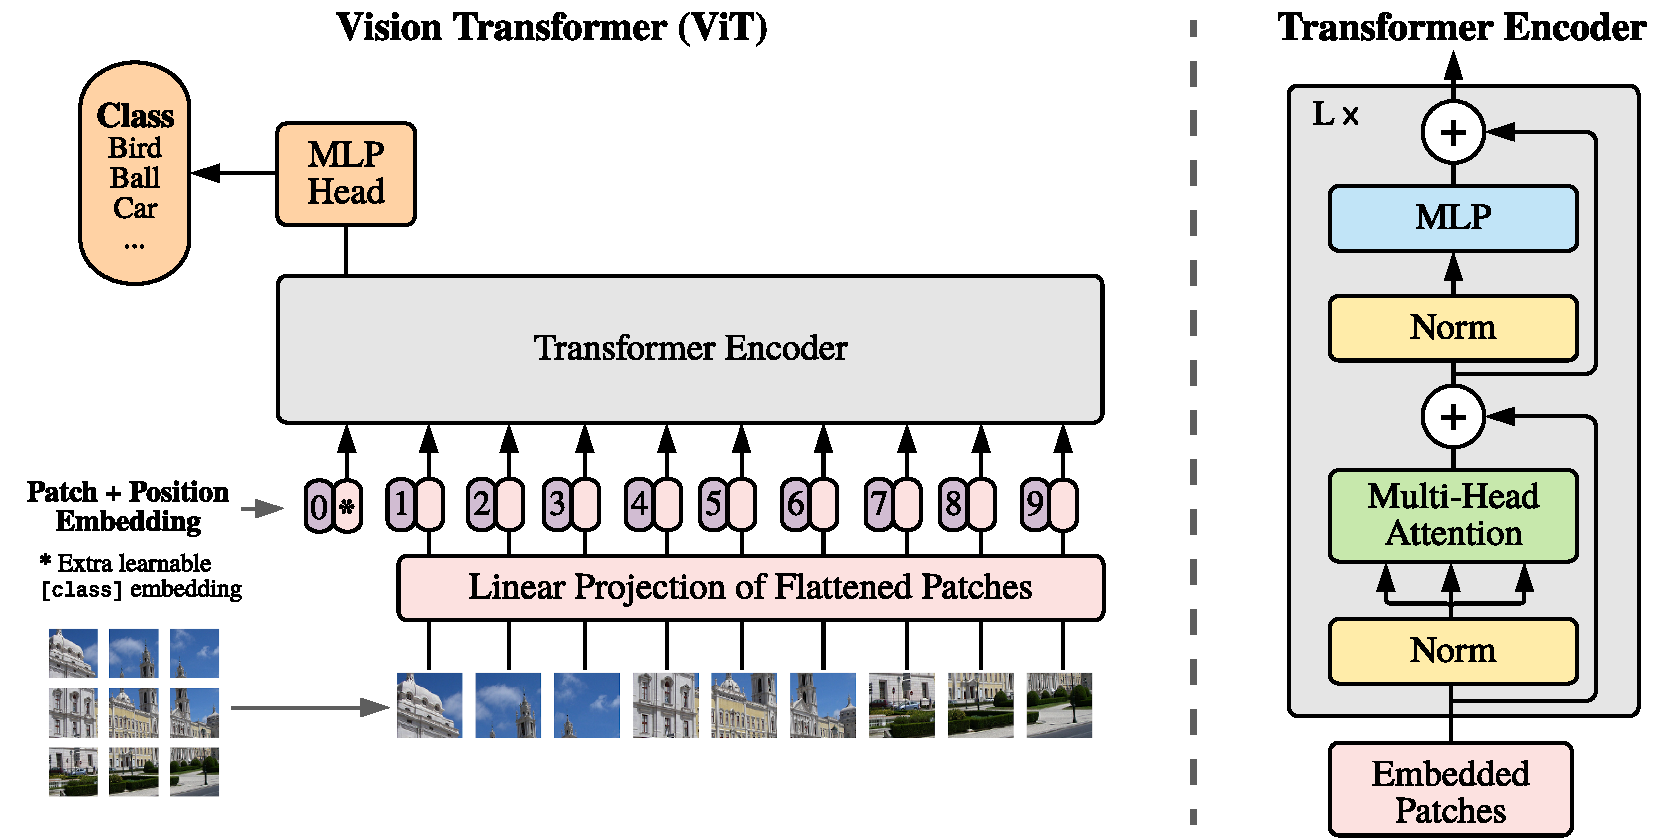
\includegraphics[width=0.8\textwidth, height=0.3\textheight, keepaspectratio]{pic/model_scheme}
    \caption{Vision Transformer 架构示意图}
    \label{fig:vit-architecture}
\end{figure}
Vision Transformer（ViT）的核心思想是将输入图像划分为一系列固定大小且不重叠的图像块（如 $16 \times 16$ 或 $32 \times 32$ 像素），
并将每个图像块展平后通过线性映射嵌入到一个低维表示空间。
随后，为每个块添加可学习的位置编码以保留空间位置信息。
通常在嵌入序列的前端插入一个可学习的 [CLS] 标记，作为可选的全局聚合位置；其末层表示的具体用途取决于下游任务，将在后文按任务类型分别说明。

这种基于图像块的表示方法使模型能够在保留局部空间结构的基础上，借助自注意力机制建模整幅图像中的全局依赖关系。

下面将结合图 \ref{fig:vit-architecture}，按照数据流动的顺序，对 Vision Transformer 的整体架构及其数据传递过程进行详细介绍：
\begin{enumerate}[label={（\arabic*）}, leftmargin=2em, labelsep=0.5em, itemsep=0pt]
\item 图像展平（Flattening）：
将输入图像 $\boldsymbol{x} \in \mathbb{R}^{H \times W \times C}$ 按照大小为 $P \times P$ 的不重叠区域划分为 $N = \frac{HW}{P^2}$ 个图像块（patch），其中 $H \times W$ 为图像分辨率，$C$ 为通道数，$P$ 为每个块的边长。

对每个图像块按空间位置展开其所有像素通道值，展平成一维向量，得到 $N$ 个向量 $\boldsymbol{x}_p^i \in \mathbb{R}^{P^2 \cdot C}$。
将这些展平后的块向量按其原始空间顺序排列，组成二维块序列，即为：
\[
\boldsymbol{x}_{p} = [\boldsymbol{x}_p^1, \boldsymbol{x}_p^2, \ldots, \boldsymbol{x}_p^N] \in \mathbb{R}^{N \times (P^2 \cdot C)},
\]
其中$\boldsymbol{x}_p^i$ 表示第 $i$ 个图像块的展平表示。

该二维块序列经下述线性投影、类别标记与位置编码处理后，才构成 Transformer 编码器的实际输入 $\boldsymbol{z}_0$。
    \item 图像块的线性投影（Linear Projection of Flattened Patches）：由于 Transformer 所有层保持固定的潜空间维度 $D$，需通过可学习的线性投影将每个图像块嵌入到 $D$ 维空间，得到由$N$个图像块组成的嵌入序列：
    \begin{equation}
        \left[\boldsymbol{x}_p^1 \boldsymbol{E}; \cdots ; \boldsymbol{x}_p^N \boldsymbol{E}\right] \in \mathbb{R}^{N \times D}, \quad \boldsymbol{E} \in \mathbb{R}^{(P^2 \cdot C) \times D}.
    \end{equation}
    \item 添加类别标记与位置编码（Patch + Position Embedding）：
    \begin{enumerate}[label={（\alph*）}, leftmargin=2em, labelsep=0.5em, itemsep=0pt]
\item 类别标记（[CLS] Token）：在嵌入序列前添加一个可学习的向量 $\boldsymbol{x}_{\text{class}}$，作为分类标记（[CLS] token），构成输入序列的首位，即：
\begin{equation}
    \left[\boldsymbol{x}_{\text{class}}; \boldsymbol{x}_p^1 \boldsymbol{E}; \cdots ; \boldsymbol{x}_p^N \boldsymbol{E}\right] \in \mathbb{R}^{\left(N+1\right) \times D}.
\end{equation}
    \item 位置编码：为保持块序列的位置信息，向每个块嵌入添加可学习的一维位置编码，构成 Transformer 的最终输入序列，即：
    \begin{equation}
        \boldsymbol{z}_0 = \left[\boldsymbol{x}_{\text{class}}; \boldsymbol{x}_p^1 \boldsymbol{E}; \cdots ; \boldsymbol{x}_p^N \boldsymbol{E}\right] + \boldsymbol{E}_{\text{pos}}, \quad \boldsymbol{E}_{\text{pos}} \in \mathbb{R}^{(N+1) \times D}.
    \label{eq:pos-emb}
    \end{equation}
    \end{enumerate}
    \item Transformer 编码器（Transformer Encoder）：由交替 $L$ 次的多头自注意力（Multi-Head Self-Attention, MSA）和多层感知机（Multi-Layer Perceptron, MLP）构成。
    每个子层前应用了层归一化（Layer Normalization，LN)，每个子层之后通过残差连接（Residual Connection）与输入相加，形成输出。

    多头自注意力（MSA）和多层感知机（MLP）在 Transformer 编码器中的每层计算过程如式\ref{eq:transformer-encoder-msa}和式\ref{eq:transformer-encoder-mlp}所示（含层归一化和残差连接）：
    \begin{align}
        \boldsymbol{z}'_l &= \text{MSA}(\text{LN}(\boldsymbol{z}_{l-1})) + \boldsymbol{z}_{l-1}, \qquad l = 1, 2, \dots, L \label{eq:transformer-encoder-msa} \\
        \boldsymbol{z}_l &= \text{MLP}(\text{LN}(\boldsymbol{z}'_l)) + \boldsymbol{z}'_l, \qquad l = 1, 2, \dots, L \label{eq:transformer-encoder-mlp}
    \end{align}
    其中 MLP 模块包含两个线性层与一个 GELU 激活函数，后者的形式为：
    \begin{equation}
        \text{GELU}(x) = x \cdot \Phi(x) = x \cdot \frac{1}{2} \left[1 + \text{erf}\left(\frac{x}{\sqrt{2}}\right)\right],
        \label{eq:GELU}
    \end{equation}
    其中 $\Phi(\cdot)$ 为标准正态分布 $\mathcal{N}(0,1)$ 的累积分布函数（CDF），$\operatorname{erf}(\cdot)$ 为误差函数。
    \item 编码器输出（Encoder Output）：经过 $L$ 层编码后，编码器输出一组与输入词元一一对应的末层表示 $\{\boldsymbol{z}^{0}_L, \boldsymbol{z}^{1}_L, \dots, \boldsymbol{z}^{N}_L\}$，其中 $\boldsymbol{z}^{0}_L$ 对应 [CLS] 标记，$\boldsymbol{z}^{1}_L, \dots, \boldsymbol{z}^{N}_L$ 对应各图像块。在每一层的多头自注意力中，所有词元相互交互，使每个表示都融合了局部图像块特征与全局上下文信息。
\end{enumerate}

ViT 编码器本身只完成对图像的特征提取，其输出表示的使用方式取决于具体的下游任务。下面分别说明两类典型任务对应的处理方式。

\textbf{（1）图像分类任务。} 取 [CLS] 标记的末层表示 $\boldsymbol{z}^{0}_L$ 作为整幅图像的全局表征——在逐层自注意力中，[CLS] 标记持续聚合所有图像块的语义信息，故可代表全图；将其经层归一化后送入分类头（MLP Head），即得到类别预测：
\begin{equation}
\boldsymbol{y} = \text{LN}(\boldsymbol{z}^{0}_L), \qquad
\hat{\boldsymbol{y}} = \text{MLP}(\boldsymbol{y}),
\end{equation}
其中 $\hat{\boldsymbol{y}} \in \mathbb{R}^{C}$ 为图像在 $C$ 个类别上的预测得分（logits），经 Softmax 归一化后得到类别概率分布，$C$ 为类别总数；分类头通常由一至两层全连接网络构成，并结合非线性激活与 Dropout。这正是 Dosovitskiy 等人提出的经典 ViT 所采用的输出方式。

\textbf{（2）序列生成任务。} 此类任务（如图像描述、图像到 LaTeX 转换）需要输出一个变长的词元序列而非单一类别，因此不使用面向全局聚合的 [CLS] 标记与分类头，而是保留全部图像块的末层表示 $\{\boldsymbol{z}^{1}_L, \dots, \boldsymbol{z}^{N}_L\}$ 作为图像的特征序列，交由自回归解码器生成目标序列：解码器在交叉注意力中以该特征序列为键（Key）与值（Value）、以已生成的词元为查询（Query），循环预测下一个词元，直至生成终止符。本文的数学表达式图像到 LaTeX 转换任务即属此类，采用 ViT 编码器与 Transformer 解码器相结合的结构；该“编码器—解码器”结构的具体设计与实现将在“模型构建”一章详细展开。
